% Additional Technical Information
\newpage
\begin{landscape}
\section{Additional Technical Information}\label{sec:appC}
\subsection{Schematics}

\begin{figure}[h!]
	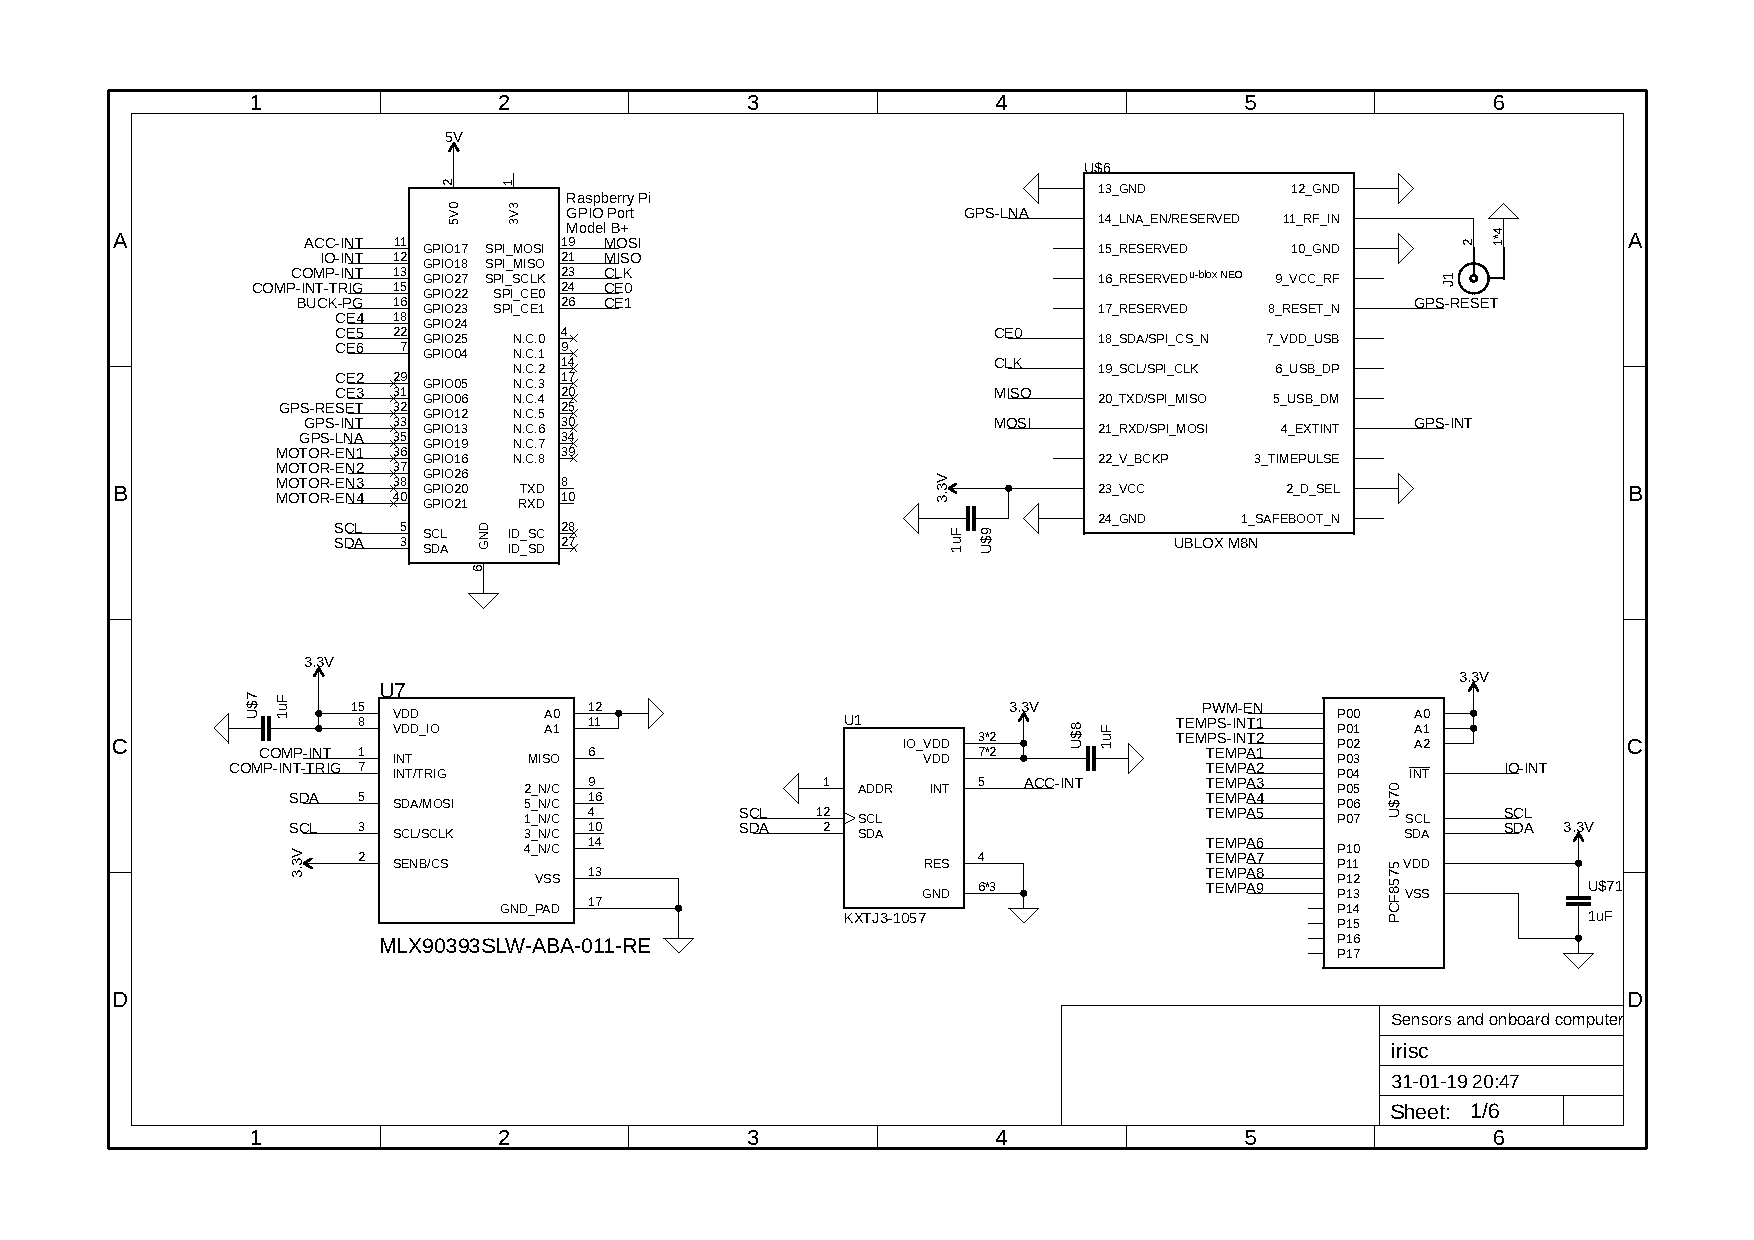
\includepdf [pages=1, angle=90]{appendix/img/schematics/irisc_v2.pdf}
\end{figure}
\newpage
\begin{figure}[h!]
		\includepdf [pages=2, angle=90]{appendix/img/schematics/irisc_v2.pdf}
\end{figure}
\newpage
\begin{figure}[h!]
		\includepdf [pages=3, angle=90]{appendix/img/schematics/irisc_v2.pdf}
\end{figure}
\newpage
\begin{figure}[h!]
		\includepdf [pages=4, angle=90]{appendix/img/schematics/irisc_v2.pdf}
\end{figure}
\newpage
\begin{figure}[h!]
		\includepdf [pages=5, angle=90]{appendix/img/schematics/irisc_v2.pdf}
\end{figure}
\newpage
\begin{figure}[h!]
		\includepdf [pages=6, angle=90]{appendix/img/schematics/irisc_v2.pdf}
\end{figure}

\newpage
\subsection{PCBs 1st iteration}
\begin{figure}[h!]
		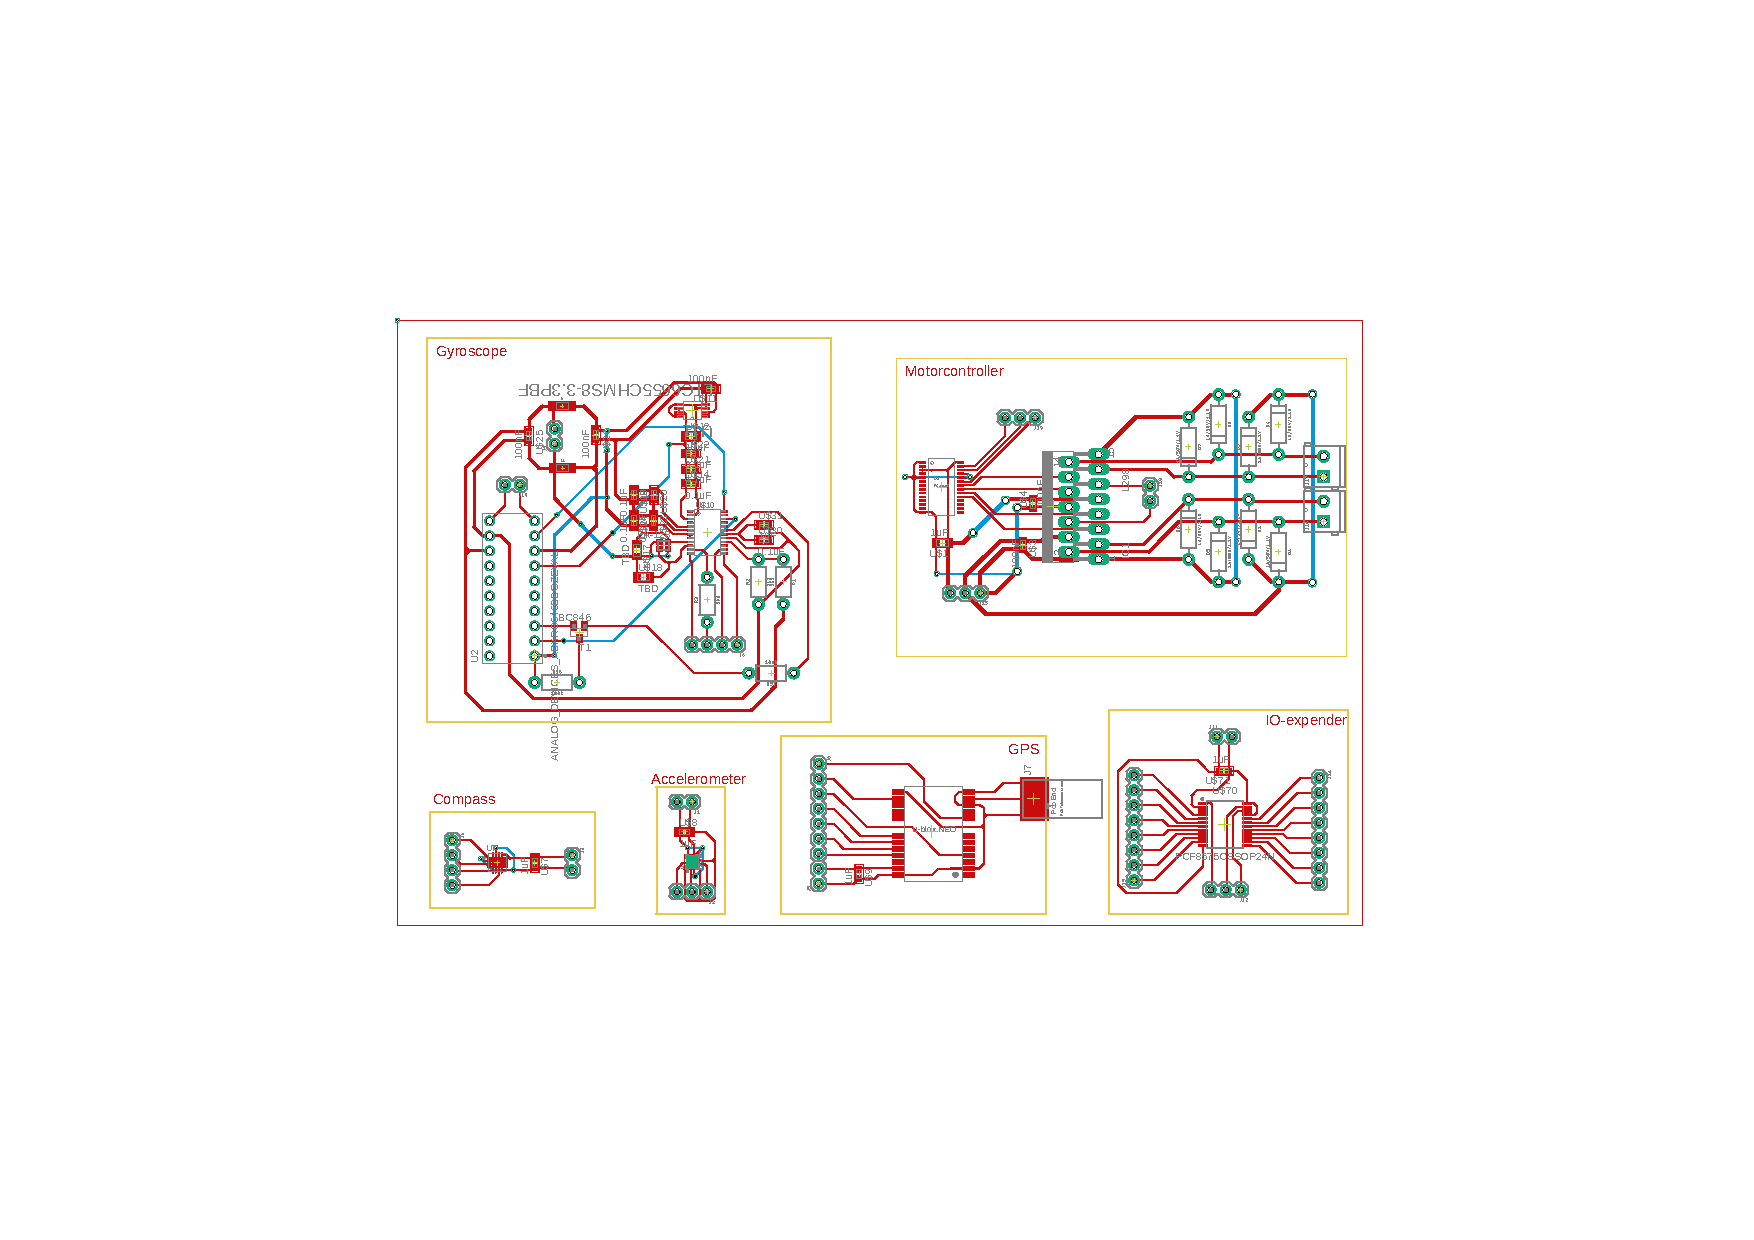
\includepdf [pages=1, angle=90]{appendix/img/pcb/irisc.pdf}
\end{figure}
\end{landscape}


\subsection{PCBs 2nd iteration}


% Highly recommend using the input function when you have a lot of stuff, it makes debugging and changing what appear in the appendix so much easier. It's also easier to edit and read. When your document starts to get big this will be the best decision you made ^^ 


% \subsection{Materials Properties}

% \input{4-experiment-design/tables/profile_material.tex}
% \bigskip
% \input{4-experiment-design/tables/wall_aluminum.tex}
% \bigskip
% \input{4-experiment-design/tables/wall_styrofoam.tex}
% \newpage
\newpage
\subsection{Manufacturing Drawings and Sketches}
\label{sec:mech_drawings}
% \begin{figure}[h!] 
% 		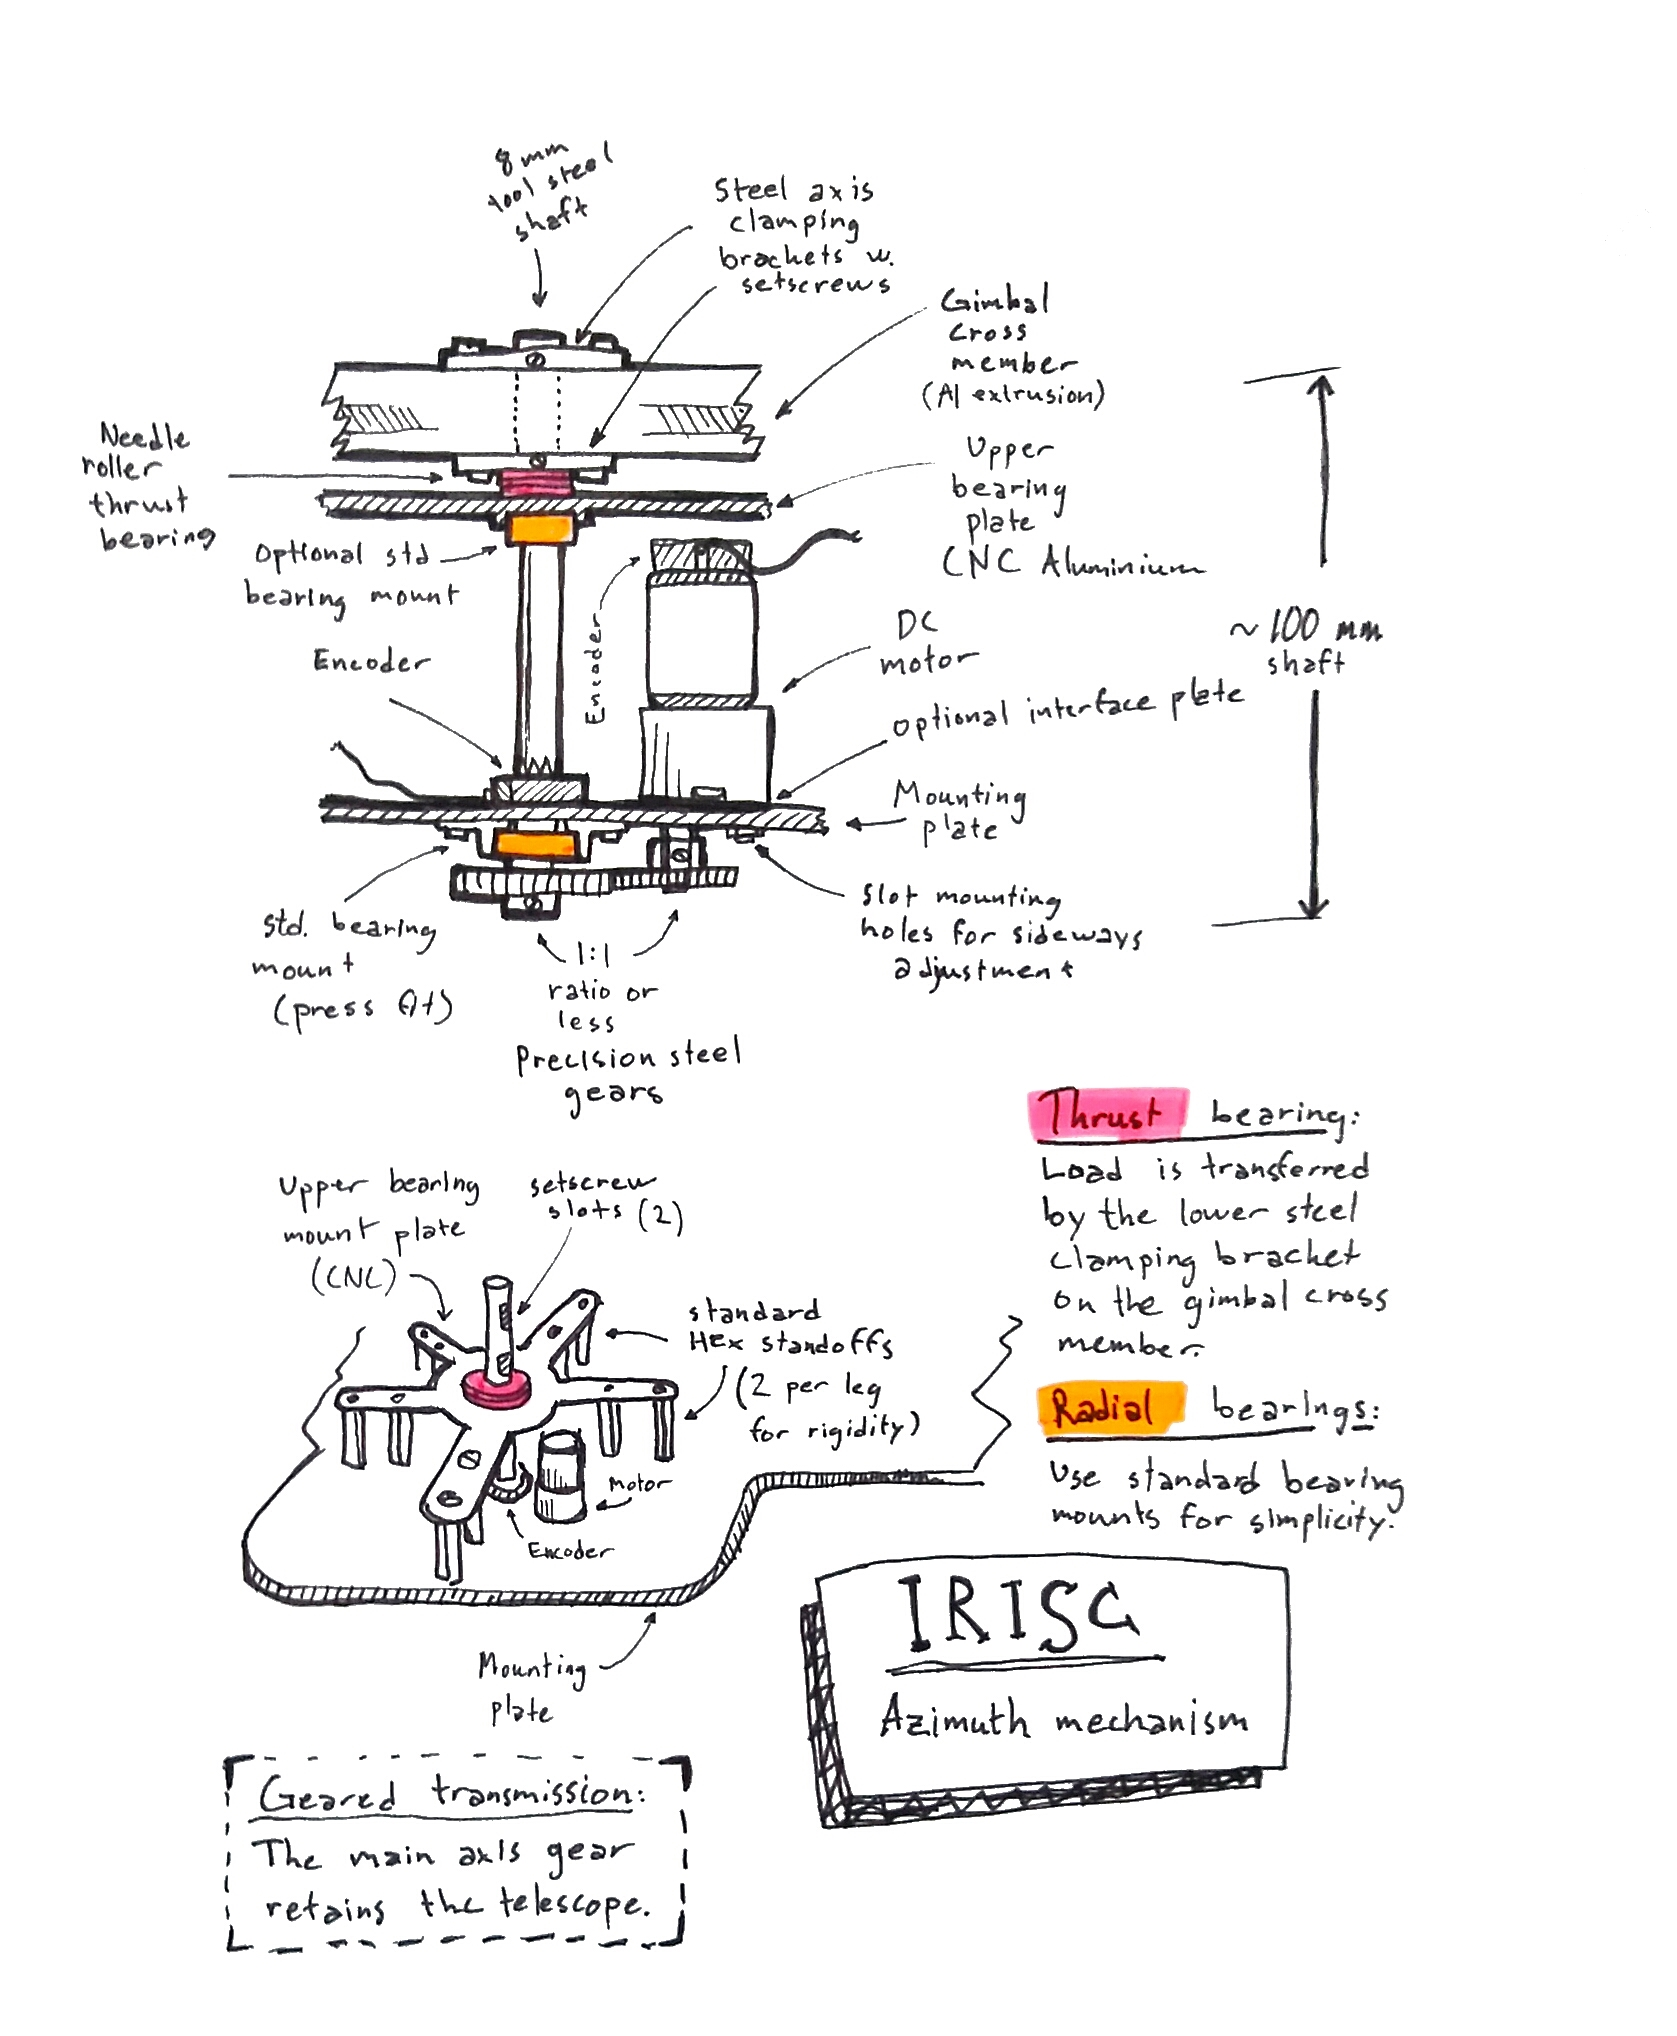
\includegraphics[width=\textwidth]{appendix/img/mechanical_sketches/azimuth_mechanism.jpg}
% 		\caption{Azimuth mechanism sketch.}
% 		\label{img:az_sketch}
% \end{figure}
% \newpage
% \begin{figure}[h!] 
% 		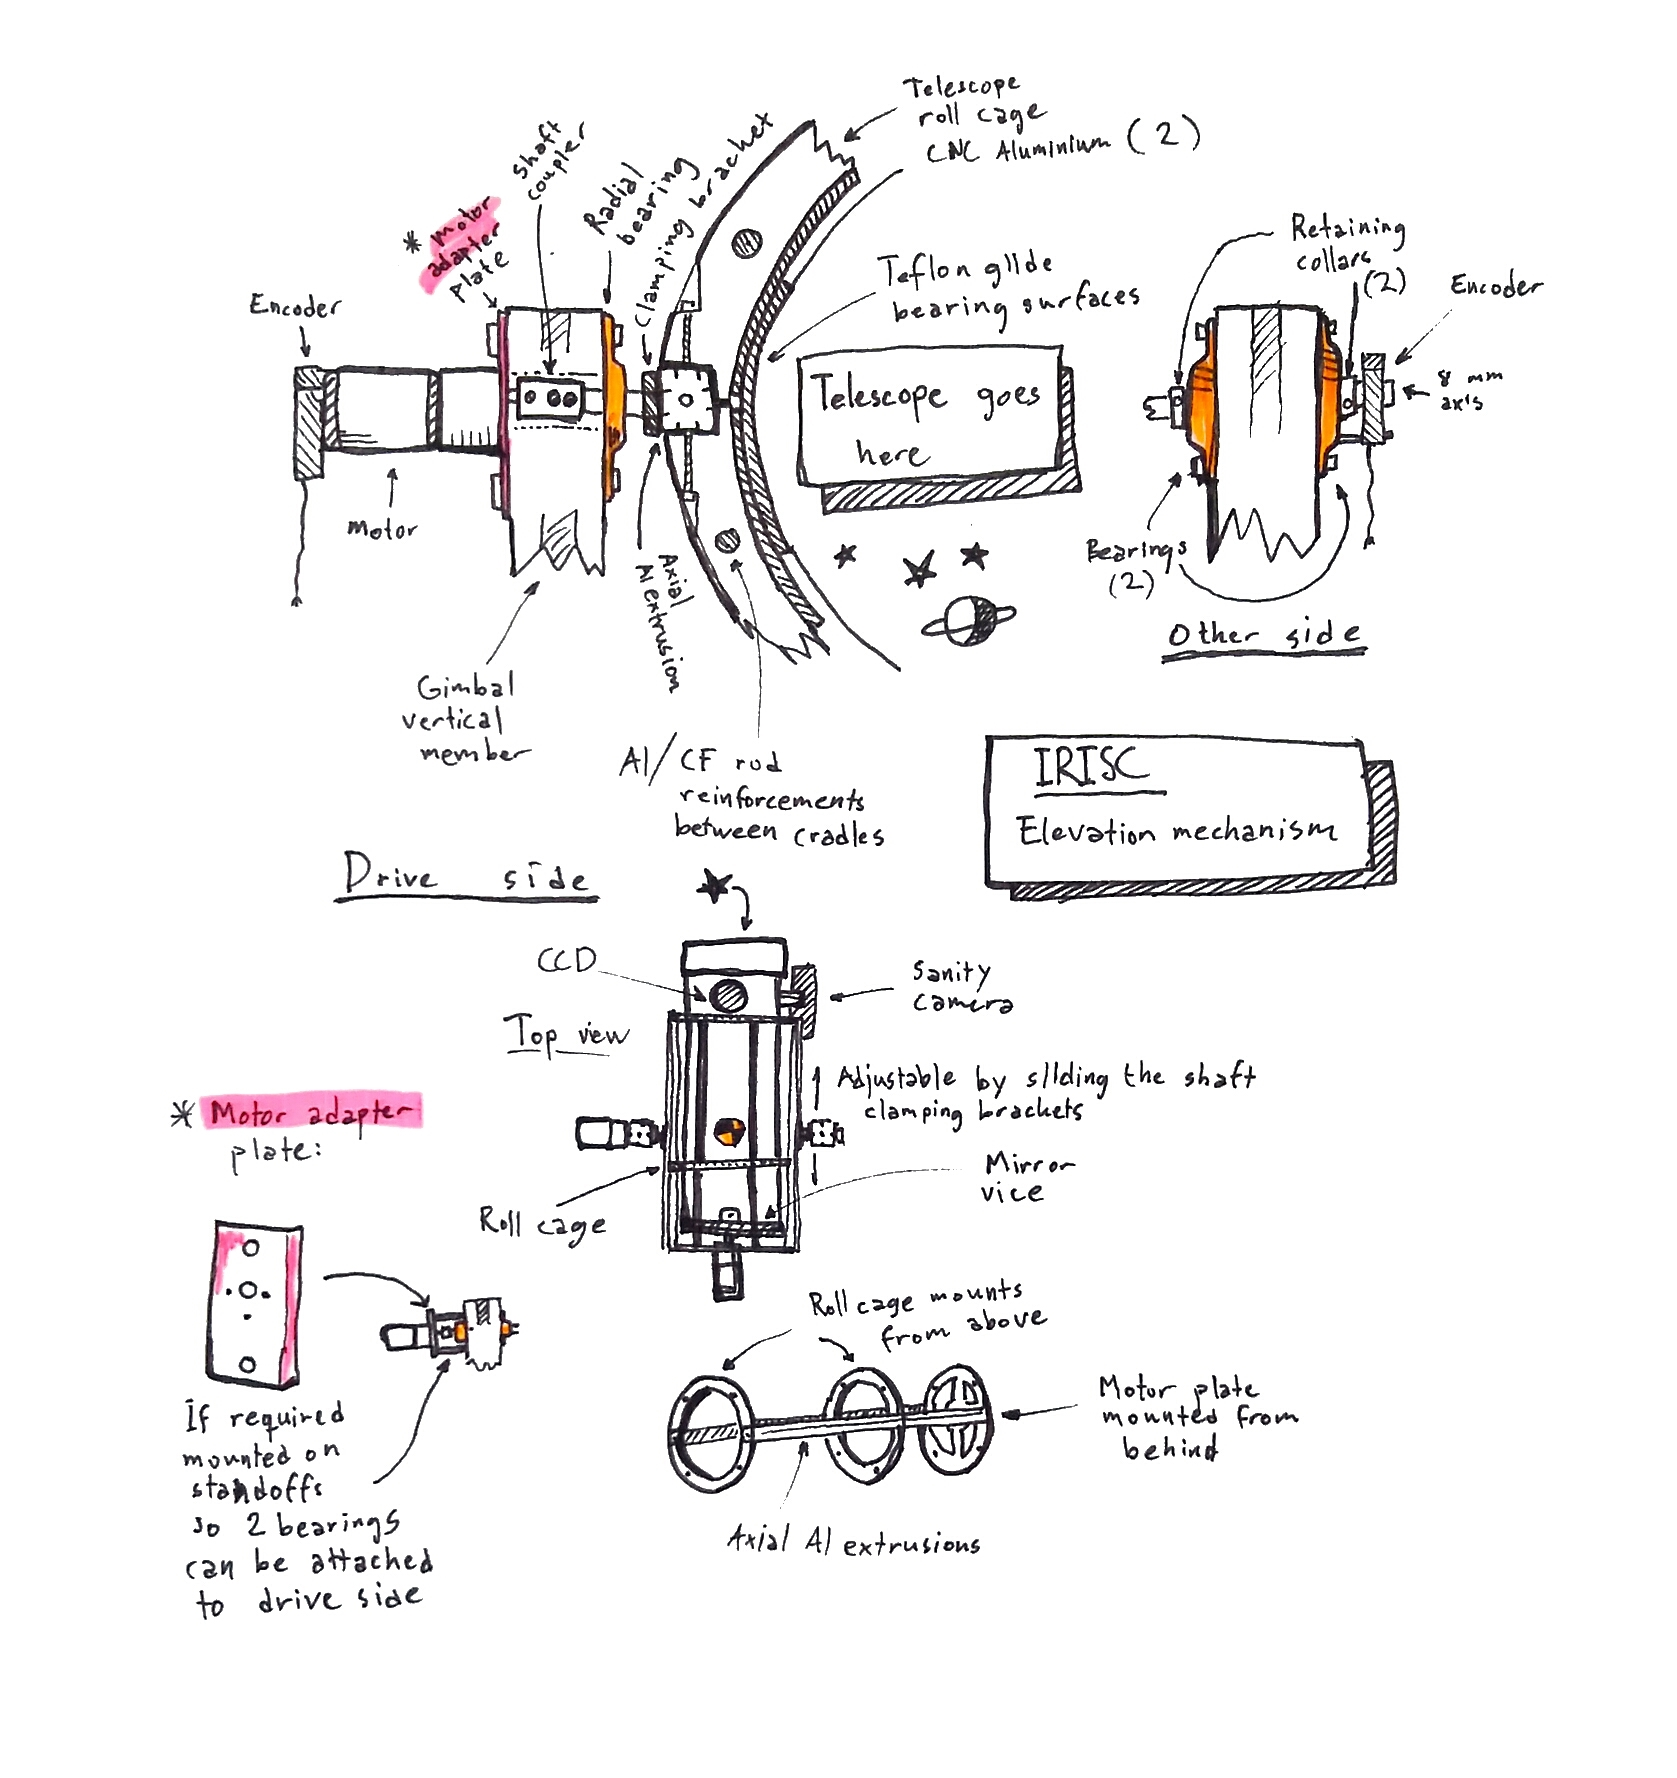
\includegraphics[width=\textwidth]{appendix/img/mechanical_sketches/elevation_mechanism.jpg}
% 		\caption{Elevation mechanism and roll cage sketch.}
% 		\label{img:el_sketch}
% \end{figure}
% \newpage
% \begin{figure}[h!] 
% 		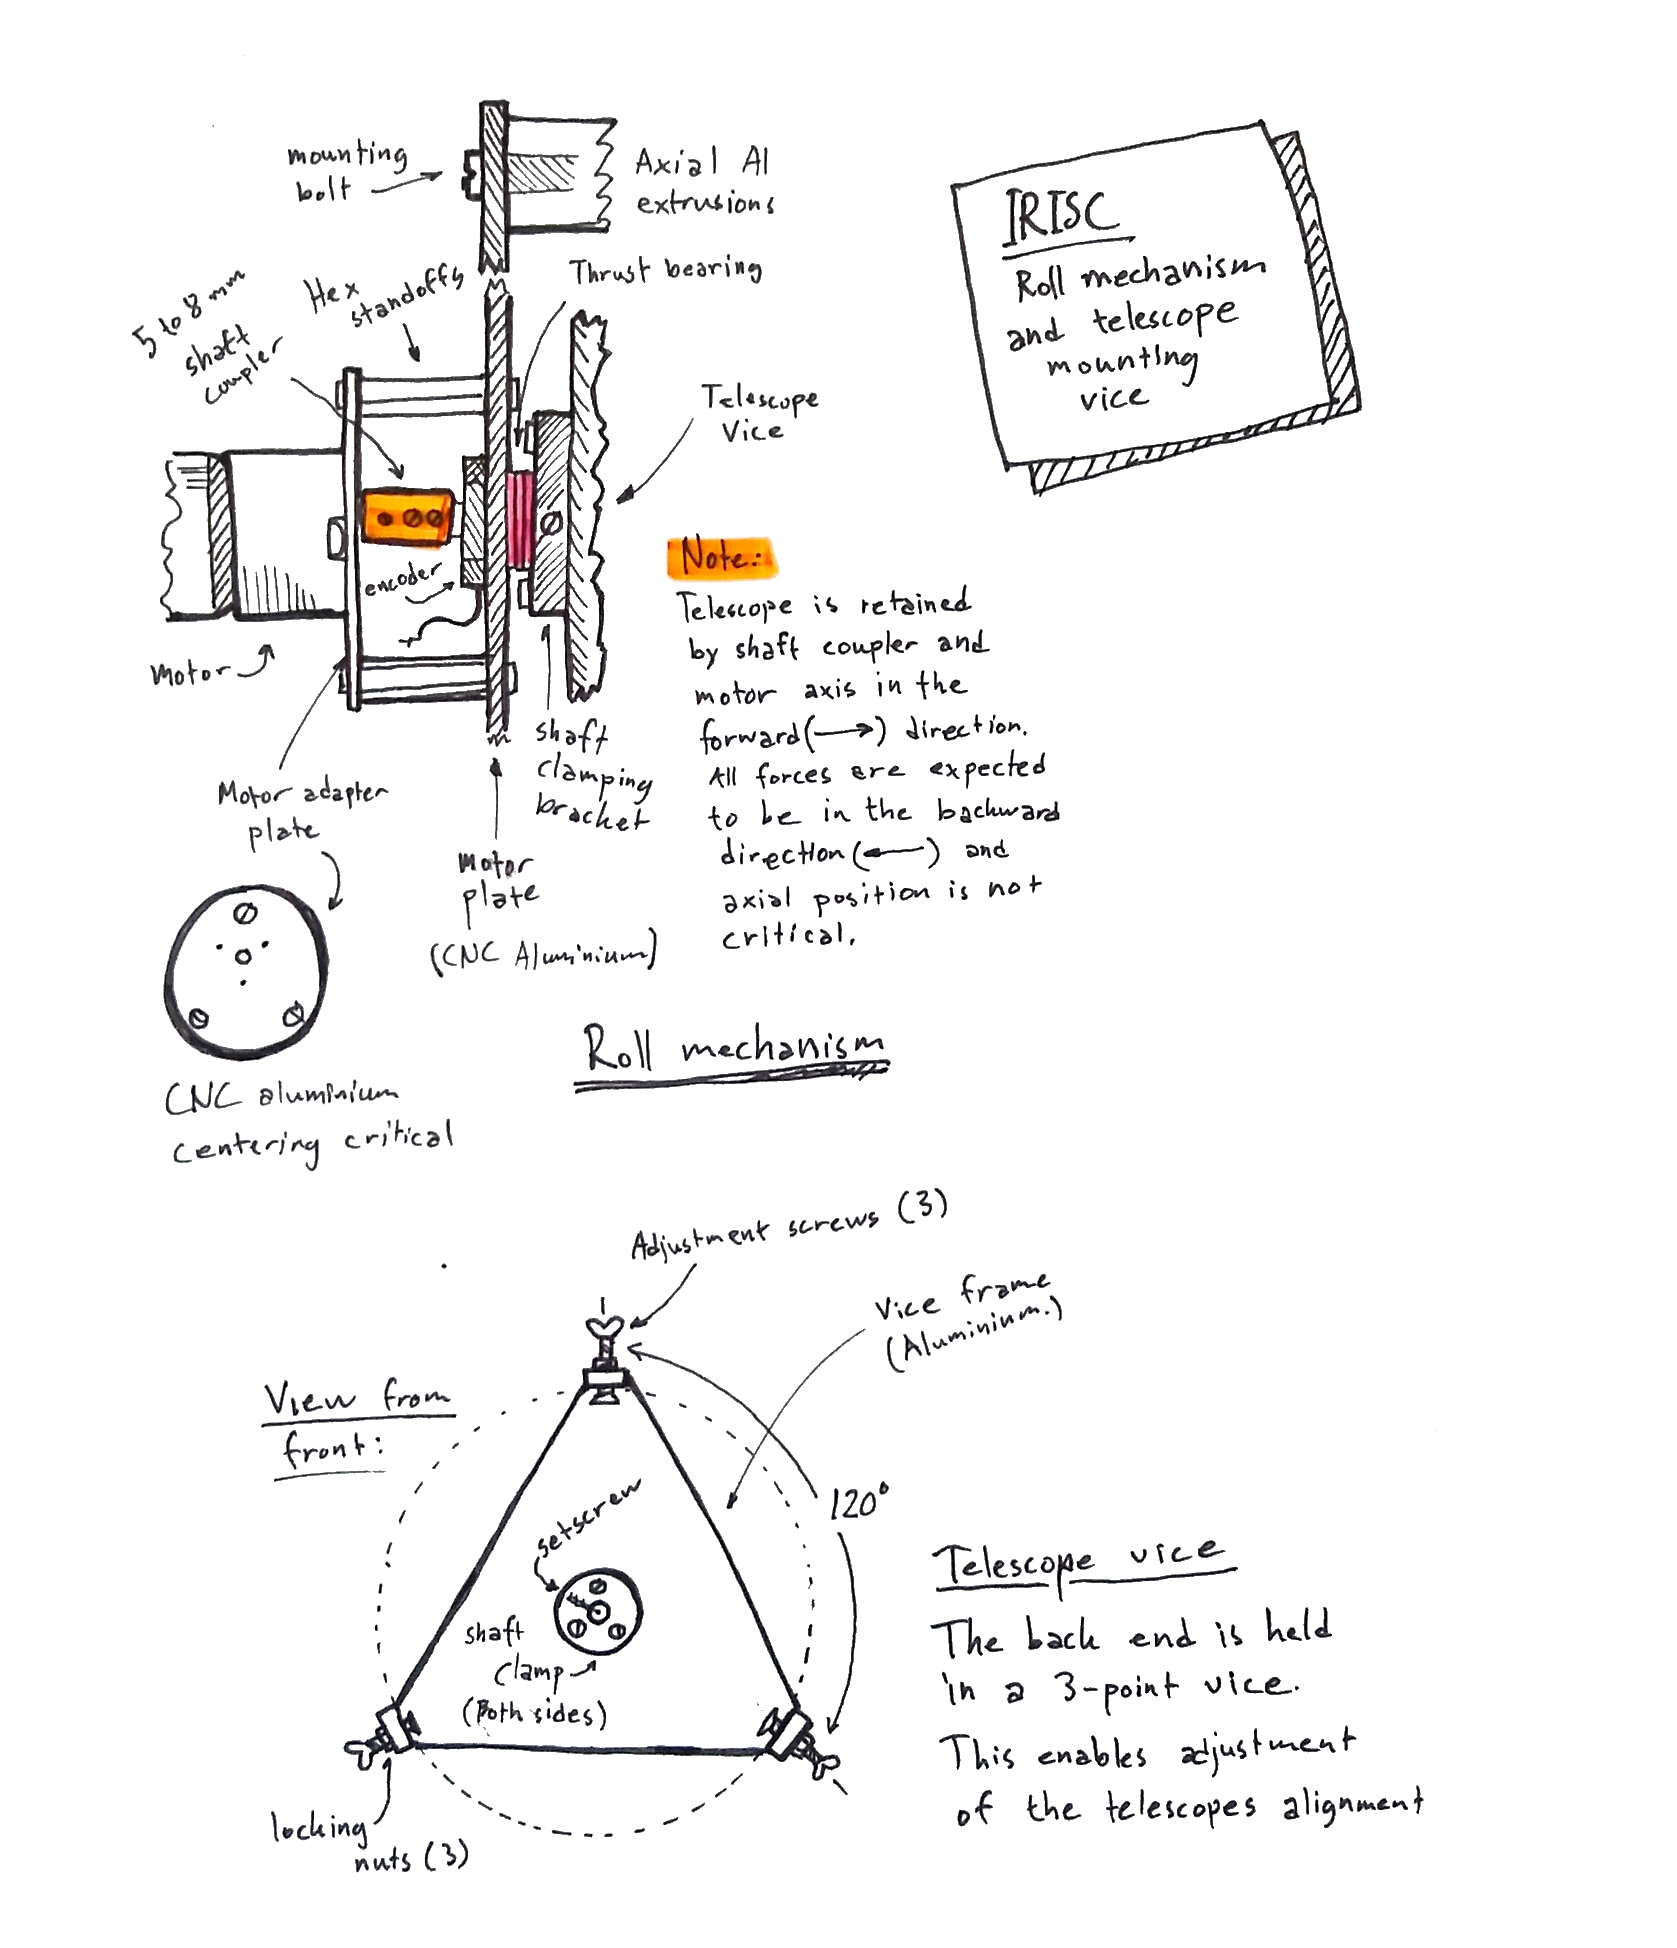
\includegraphics[width=\textwidth]{appendix/img/mechanical_sketches/roll_mechanism.jpg}
% 		\caption{Roll mechanism and telescope retaining vice sketch.}
% 		\label{img:roll_sketch}
% \end{figure}

\begin{figure}[H]
	\centering 
	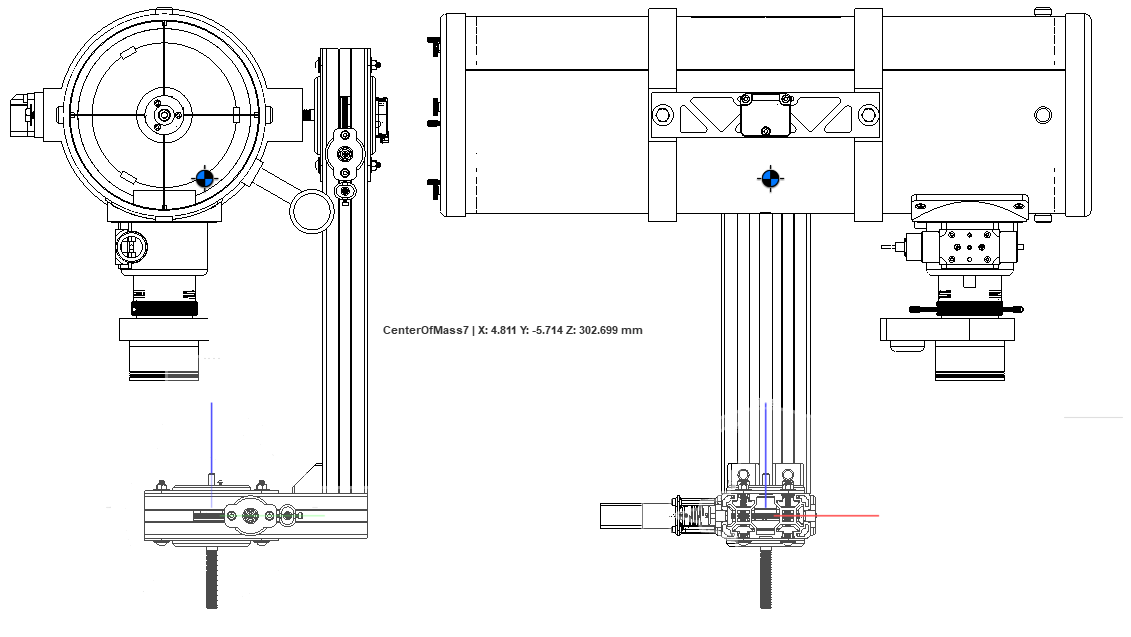
\includegraphics[scale=0.6]{4-experiment-design/img/mechanical/COM.png}
	\caption{Gimbal center of mass estimation.}
	\label{fig::mechanical::COM}
\end{figure}

\begin{landscape}
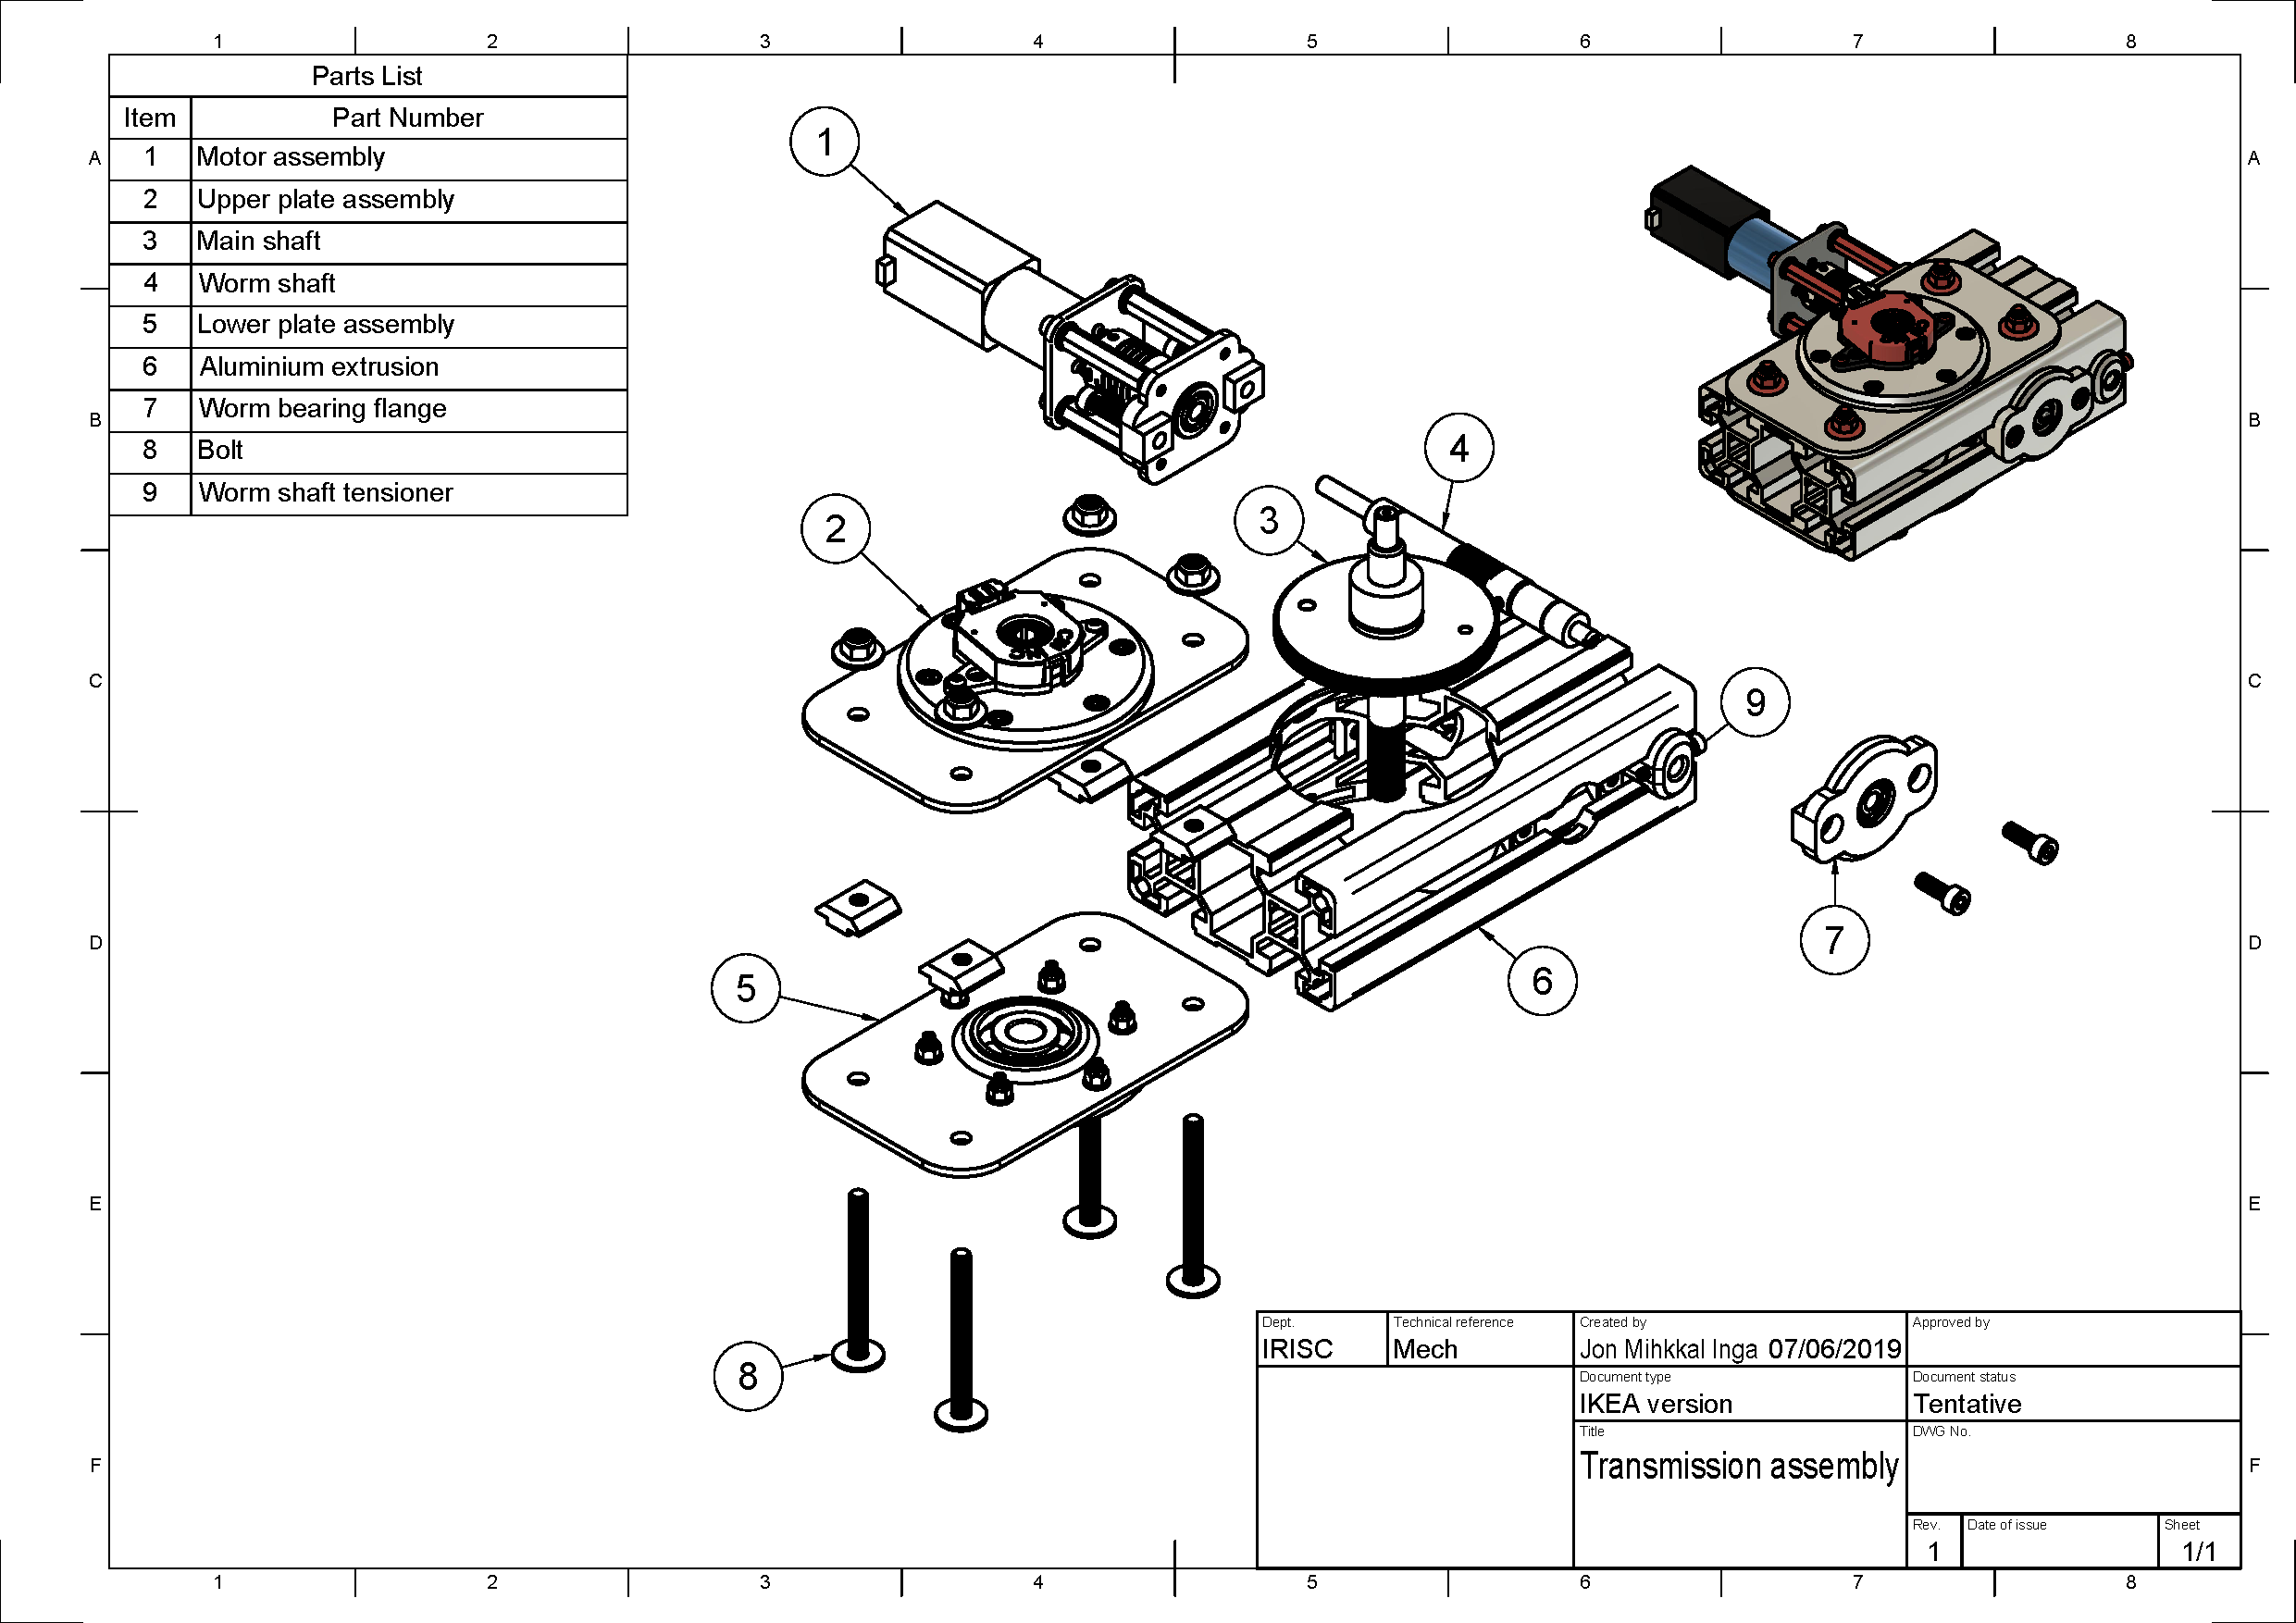
\includegraphics[scale=0.5]{appendix/img/mechanical_sketches/Transmission_Assembly.pdf}

\includegraphics[scale=0.5]{appendix/img/mechanical_sketches/Moments v1.pdf}

\end{landscape}
\newpage
% \includepdf[scale=1,pages={1,2,3,4,5,6,7,8,9,10,11,12,13,14,15,16,17,18,19,20,21,22,23,24,25,26,27,28,29,30,31,32,33,34,35,36}]{appendix/pdf/manufacturing-drafts.pdf}



% \newpage
% %\appendix
\begin{landscape}
\subsection{Software Sequence Diagram} \label{sec:XXX}

% \subsubsection{Air Sampling Control Object Sequence diagrams}
% \begin{figure}[H]
%     \centering
%     \includegraphics[height=0.9\textwidth]{appendix/img/softwareDiagrams/Sequance-Diagram-descent-Mode.jpg}
%     \caption{Sensor Object in Normal - Descent Mode.}
%     \label{sensorc}
% \end{figure}
\end{landscape}
% \newpage
% \subsection{Software Interface Diagram} \label{sec:XXXX}
% \subsubsection{Sensor Object Interface Diagram} %\label{}
% \begin{figure}[H]
%     \begin{align*}
%       \includegraphics[width=1\linewidth]{appendix/img/softwareDiagrams/interface_diagram-1-2.jpg}
%     \end{align*}
%     \caption{Sensor Object Interface Diagram.}
%     \label{fig:C1}
% \end{figure}


% \newpage
% \subsection{PCB Schematics}
\label{sec:pcbSchematics}

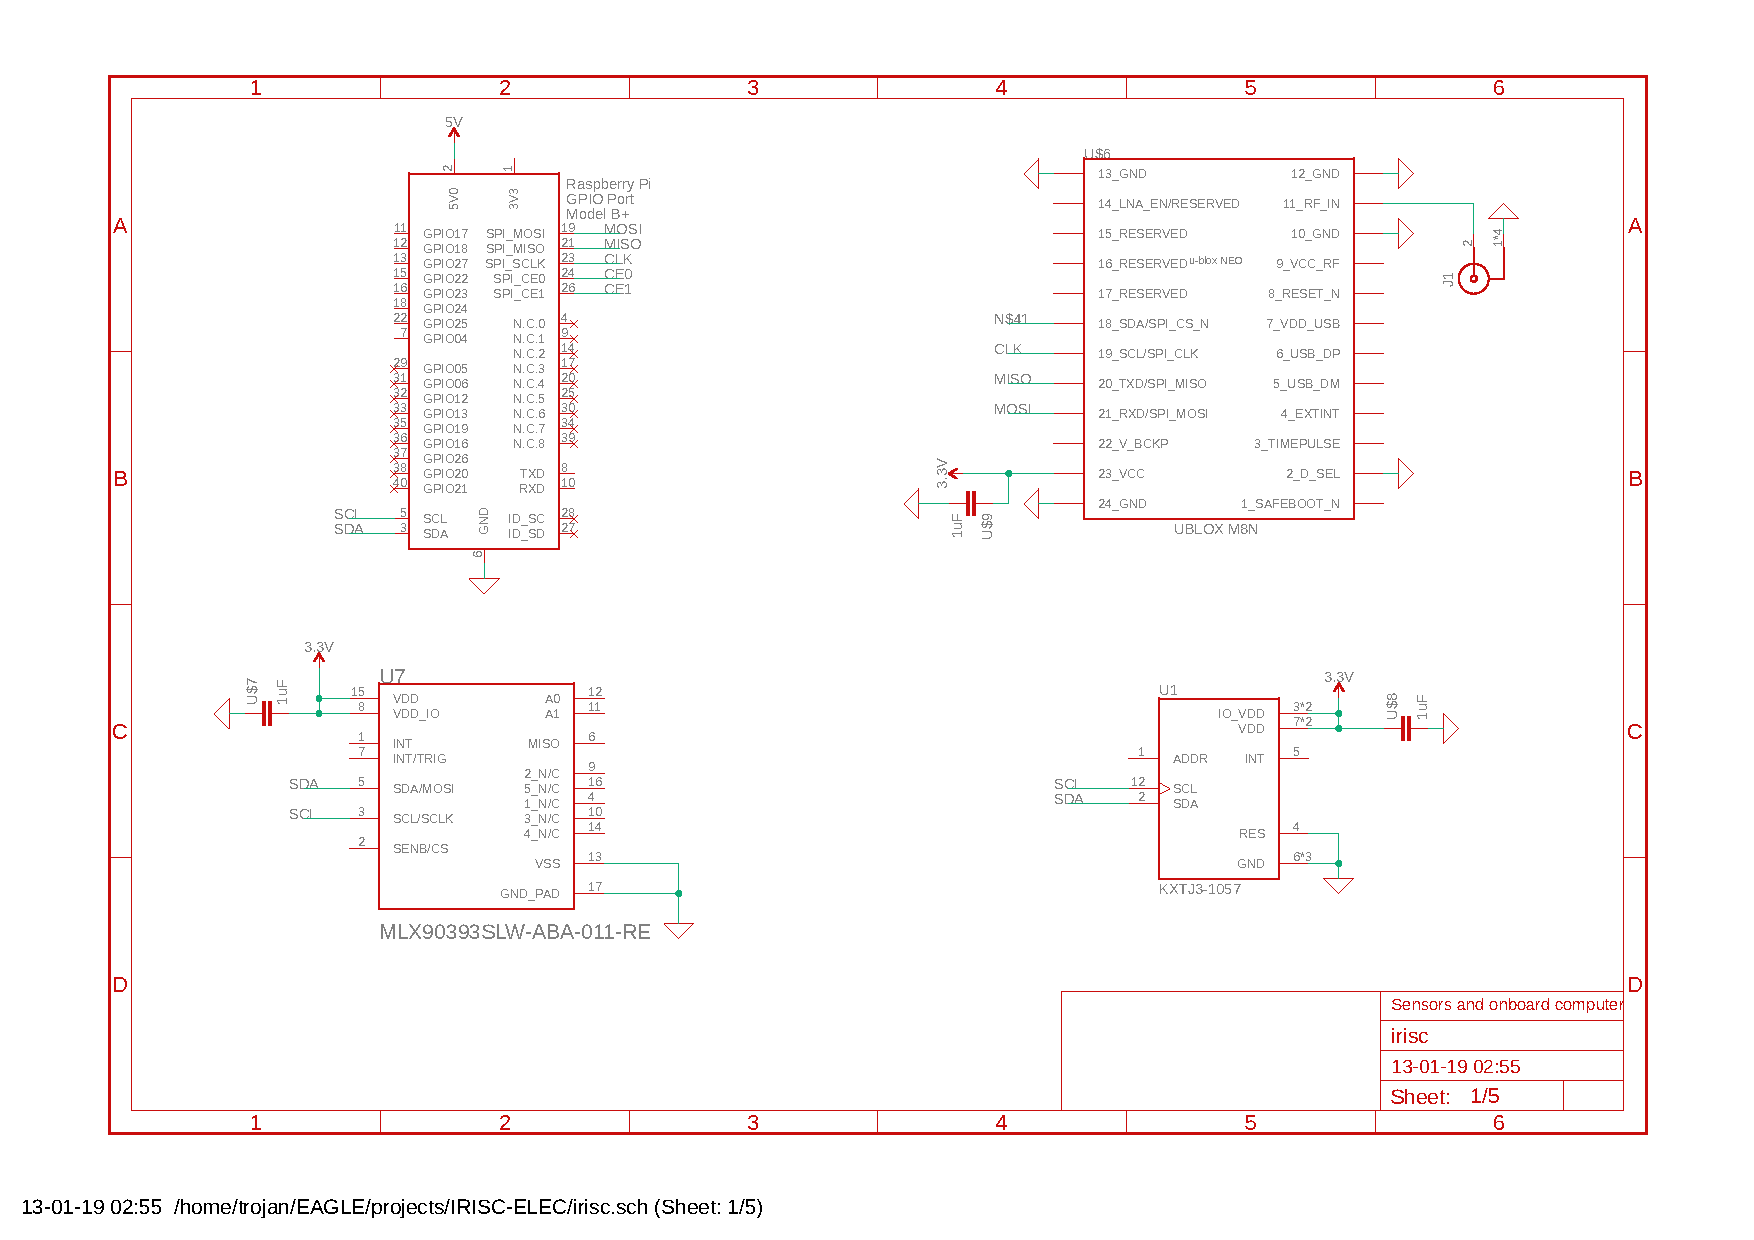
\includepdf[pages=-]{appendix/img/schematics/irisc.pdf}
% \newpage


% Same as with the experiment review PDFs but this time for data sheets of main/critical components

\clearpage
\subsection{\hl{GPS Test}}
\label{app:gps_test}
\subsubsection*{Introduction}
\vspace{-.3cm}
A test is performed to verify that the positioning provided by the GPS receiver is precise enough to fit the requirements from the control system. All three axes (latitude, longitude, altitude) are tested. Note that the defined requirement regarding the accuracy of the GPS data (P.10) exceeds our needs. See further discussion regarding this point in the discussion subsection. 

This test is performed during a car ride from Skärgårdsstad to Grebbestad on the east and west coasts of Sweden respectively.

\subsubsection*{Method \& Setup}
\vspace{-.3cm}
The GPS receiver is connected to a Raspbery Pi 4B (RPi) and the antenna is taped to the window of the car as shown in figure \ref{gps_pos}. All output from the receiver is logged during the entire journey and saved for analysis.

\begin{figure}[H]
	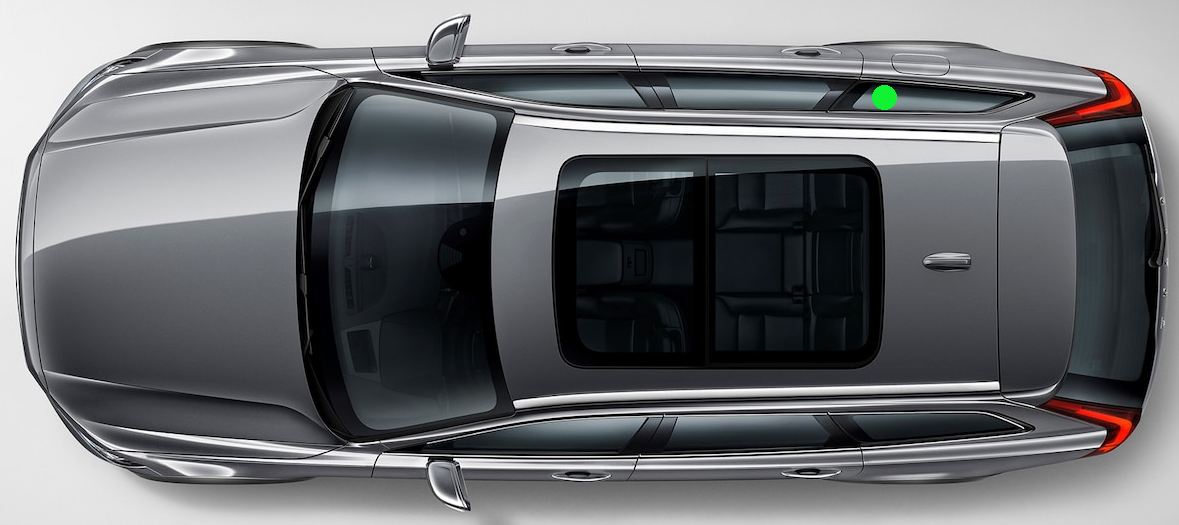
\includegraphics[width=\textwidth]{appendix/img/test-results/gps_pos.png}
	\caption{The green dot shows the position of the gps receiver on the car.}
	\label{gps_pos}
\end{figure}

Due to the lack of access to matching GPS data that is known to be accurate, the latitude and longitude data is plotted in Google MyMaps and compared with satellite imaging. Reference altitude data is produced by \url{https://www.gpsvisualizer.com/elevation} from NASA SRTM1 observational data by fetching altitude from measured latitude and longitude data.

\subsubsection*{Result}
\vspace{-.3cm}
\paragraph{Horizontal Position}
The GPS data plotted on Google MyMaps can be found here: \href{https://drive.google.com/open?id=1pnCSIn2Zt-UFfs62nne9t4oyZEai1yfZ&usp=sharing}{link}. There are three breaks in the data set due to periods where the car engine was off. Data collection during this time was not possible due to the RPi being powered by the car (and the car having a stupid ignition system). \\

As the analysis isn't numerical, an exact accuracy verification cannot be achieved. However, the data points rarely stray off of the roads and if so then only by a few meters on the right side of the road, which is to be expected as the receiver was placed on the right side of the car. Assuming the satellite imaging provided by Google is correct, the horizontal error can be roughly estimated to be within 5 meters.

\paragraph{Vertical Position}

Figure \ref{alt_comp} shows the difference between the measured and generated altitude (measured - generated). This is distributed around -5.7\,m with a standard deviation of 5.2\,m. The magnitude of the largest error encountered is 36.1\,m. Figure \ref{alt_plot} shows both sets of altitude data along the traveled path.

\begin{figure}[H]
	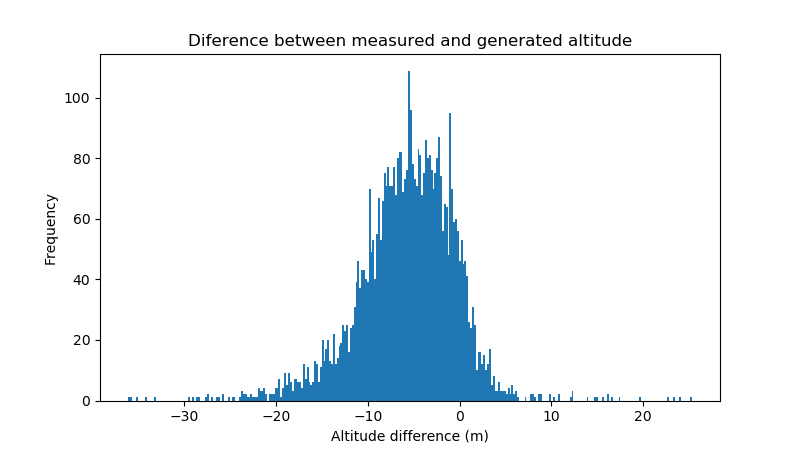
\includegraphics[width=\textwidth]{appendix/img/test-results/gps_alt_comp.png}
	\caption{The distribution of the difference measured - generated altitude.}
	\label{alt_comp}
\end{figure}

\begin{figure}[H]
	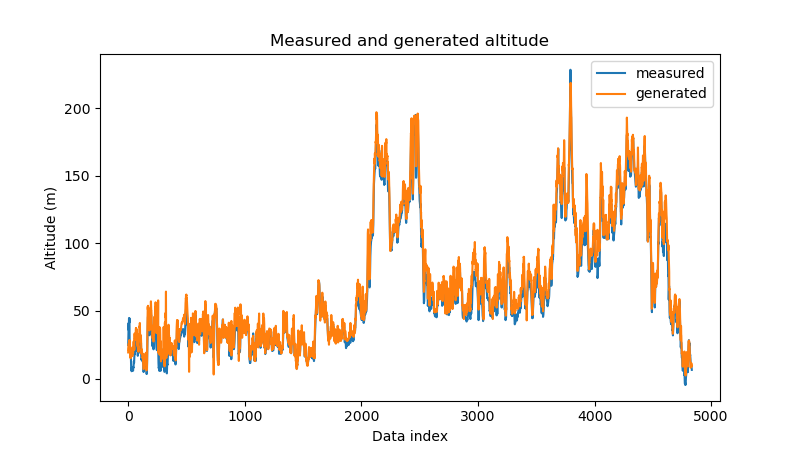
\includegraphics[width=\textwidth]{appendix/img/test-results/gps_alt_plot.png}
	\caption{The altitude along the path as measured and generated data.}
	\label{alt_plot}
\end{figure}

\subsubsection*{Discussion}

The GPS data is mainly required for two things: calculating the sidereal time of the gondola, and monitoring the altitude. An accuracy of 5 meters for either of these purposes is very small. An error one order of magnitude greater would have a minimal effect on any further calculations. For this reason, the requirement specified in the SED is ignored and the accuracy of GPS receiver is deemed to be adequate.\\

There is a bug in the current implementation of the GPS system. If the receiver doesn't have the correct message type ready (GGA) the GPS poller becomes a blocking wait, causing unnecessary usage of system resources. However this bug has only occurred during a hardware error, e.g. one pin disconnecting or a clock speed error (upgrading from the RPi 3B+ to the RPi 4B increases CPU clock speed while using the same library which causes the SPI delay times to be too short). The test described above can also act as an endurance test of roughly 6 hours in total during which this error didn't occur.
\clearpage
\subsection{Camera Software Test}
\label{app:camera_software_test}
\subsubsection*{Introduction}

Much of the camera functionality is verified by analysis and compared with software provided by ZWO (ASICAP). For example the library written in the IRISC software produces an image of the correct format with the correct file size and the correct header content (more header content can still be added in necessary). To analyze noise differences two tests are made:

\begin{enumerate}
    \item The IRISC software is compared with the ASICAP software provided by ZWO.
    \item Connecting the camera via USB 2 and USB 3 is compared using the IRISC software.
\end{enumerate}

\subsubsection*{Method \& Setup}

The telescope is set up on vibration dampening legs facing a building wall roughly 50 meters away.

For test 1, the camera is connected to a laptop over USB 3. Next the IRISC software in run which captures ten images. That is followed by capturing ten images using ASICAP.  For test 2, the camera is connected to a RPi 4B through USB 3. The IRISC software then captures ten images. The camera is then disconnected and reconnected through a USB 2 port and another ten images are captured after a few seconds to let any vibrations caused by moving the table to die down. Two comparisons are made in each test:

\begin{enumerate}
    \item The sets of images from each software are averaged pixel wise and a difference between the means is calculated. The mean and standard deviation of the distribution of the pixels in this diff image is analyzed to find if any noise is added consistently. 

    \item The differences between the images in each set is investigated.  This is done by subtracting the mean pixel wise from each image and analyzing the standard deviation of the resulting distribution.
\end{enumerate}

\subsubsection*{Result}

\paragraph{Test 1, Comparison 1 (T1C1)}\,\\

The result from the first comparison follows a normal distribution, $ N( -0.393, 21.4^2 ) $.

\paragraph{Test 1, Comparison 2 (T1C2)}\,\\

The images from the IRISC software follow the normal distribution $ N( 0, 43.2^2 ) $.
The images from ASICAP follow the normal distribution $ N( 0, 43.4^2 ) $.
The total time required to capture the images was 6 and 32 seconds respectively for the two softwares.

\paragraph{Test 2, Comparison 1 (T2C1)}\,\\

The distribution in T2C1 can be estimated with a heavily skewed normal distribution, $ N( 349, 82.2^2 ) $ with a skewness of 90.2. Figure \ref{usb_comp} shows this distribution.

\begin{figure}[H]
    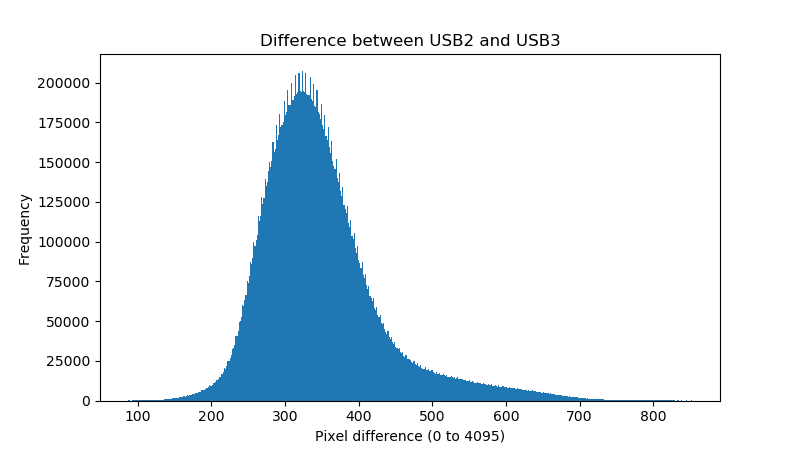
\includegraphics[width=\textwidth]{appendix/img/test-results/camera_software_test.png}
    \caption{The distribution of the pixel wise difference USB 2 - USB 3 for image capturing.}
    \label{usb_comp}
\end{figure}

\paragraph{Test 2, Compatison 2 (T2C2)}\,\\

The images taken over USB 2 and 3 follow the distributions $ N( 0, 59.6^2 ) $ and $ N( 0, 41.1^2 ) $ respectively. The distributions have a slight positive skew of 0.141 and 0.025 respectively. The total time required to capture the images was 30 and 10 seconds respectively for the two interfaces.

\vspace{-.3cm}
\subsubsection*{Discussion}

The mean difference between the images captured using IRISC software and using ASICAP of -0.393 is within margin of error. Considering that the sensor has a 12 bit ADC resulting in 4096 possible values, a standard deviation of 41 corresponds to $1\%$ of the maximum pixel value. Since there is a small time difference between each image capture and since the sensor isn't perfect, there will be some random noise added. Therefore the standard deviation of T1C1 can be assumed to be independent of the software used. Since the standard deviations of T1C2 are almost equal, it can be concluded that the IRISC software doesn't introduce any noise when compared to ASICAP.\\

\vspace{-.1cm}
The result from T2C1 and the almost 50\% higher standard deviation in T2C2 shows that there is a lot of noise added when the camera is operated over USB 2. This is due to the camera not having an onboard memory buffer as mentioned in section 6.8 in the camera manual (\href{https://astronomy-imaging-camera.com/manuals/ASI183\%20Manual\%20EN.pdf}{link, page 12}). This means that the data is read directly from the sensor. Therefore, the slower the data is read the more noise will be added. Because of this we will either need to upgrade to the Pro version of the camera or upgrade to a RPi 4B to avoid noise since the currently used RPi 3B+ does not have USB 3 capabilities. Upgrading to the Pro camera version is not recommended due to costs but it is noteworthy that there is probably noise added without memory buffer even when using USB 3.
% \includepdf[scale=0.75,pages={3},pagecommand=\subsection{Tube}]{appendix/pdf/Rtx-Catalog015-6_Tubing.pdf}

% \includepdf[scale=0.75,pages={4},pagecommand=\subsection{AAC Manifold Valve}]{appendix/pdf/VDW_A_EU.pdf}
% \includepdf[scale=0.75,pages={7},pagecommand=\subsection{AAC Flushing Valve and CAC Valve}]{appendix/pdf/VDW_B_EU.pdf}
% \includepdf[scale=0.75,pages={8,9}]{appendix/pdf/VDW_B_EU.pdf}

% \includepdf[scale=0.75,pages={4},pagecommand=\subsection{Pump}]{appendix/pdf/DataSheet_NMP830_850_E005_web.pdf}

% \includepdf[scale=0.75,pages={1},pagecommand=\subsection{Airflow Sensor}]{appendix/pdf/honeywell-sensing-airflow-awm50000-series-catalog-pages.pdf}
% \includepdf[scale=0.75,pages={2,3,4}]{appendix/pdf/honeywell-sensing-airflow-awm50000-series-catalog-pages.pdf}

% \includepdf[scale=0.75,pages={1},pagecommand=\subsection{Static Pressure Sensor}]{appendix/pdf/Gems_3500_eng_tds.pdf}
% \includepdf[scale=0.75,pages={2,3}]{appendix/pdf/Gems_3500_eng_tds.pdf}